\documentclass[11pt]{article}

\usepackage{light}
\usepackage{tikz}
\usepackage{enumerate}
\usepackage{paralist}

\hidesolutions
%\showsolutions

\newcommand{\edge}[2]{#1\text{---}#2}
\newcommand{\eqdef}{:=}
\newcommand{\suchthat}{\text{ s.t. }}
\newcommand{\rationals}{\mathbb{Q}}
\newcommand{\reals}{\mathbb{R}}
\newcommand{\integers}{\mathbb{Z}}
\newcommand{\naturals}{\mathbb{N}}
\newcommand{\union}{\cup}
\newcommand{\intersect}{\cap}

%\newcommand{\divides}{\mid}
%\newcommand{\ceil}[1]{\left\lceil#1\right\rceil}
%\newcommand{\floor}[1]{\left\lfloor#1\right\rfloor}

\newcommand{\arc}[2]{#1\!\longrightarrow\!#2}

\newcommand{\mfigure}[3]{\bigskip\centerline{\resizebox{#1}{#2}{\includegraphics{#3}}}\bigskip}

\begin{document}

\recitation{9}{October 8, 2014}



When you search for a broad term (e.g., ``mathematics') on Google, there are typically millions of matches; many webpages contain the word mathematics! In order to give useful results, Google needs to find a good way of ranking these results.

The success of Google is founded on a good way to do this, using the digraph structure of the web. The ``PageRank'' algorithm was invented by Larry Page and Sergey Brin. There are a lot more complications than we'll discuss here, but we will be able to understand the core of the idea.

\subsection*{The web graph}

We can construct a digraph from the web very easily: the vertices of the graph are webpages, and there is a directed edge from webpage $i$ to webpage $j$ if $i$ has a link to $j$. Here are two (very small) web graphs:

\begin{center}
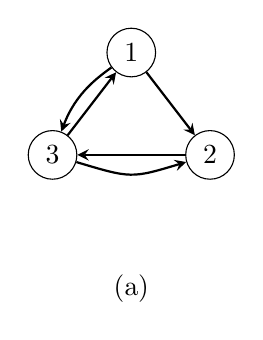
\begin{tikzpicture}
    \begin{scope}[every node/.style={circle,draw}]
    
    \node[draw] (v3) at (0,0.7) { 3 };
	\node[draw] (v2) at (2,0.7) { 2};
    \node (v1) at (1,2) { 1 };
\end{scope}

\node (la) at (1, -1) { (a) };

\begin{scope}[>=stealth,->,thick]
   \draw[->] (v1) edge (v2);
   \draw[->] (v2) edge (v3);
   \draw[->] (v3) edge (v1);
  \draw (v1) .. controls (0.6,1.7) and (0.3,1.5) .. (v3) ;
  \draw (v3) .. controls (1,0.4)  .. (v2);
\end{scope}
\end{tikzpicture}
\hspace{5cm}
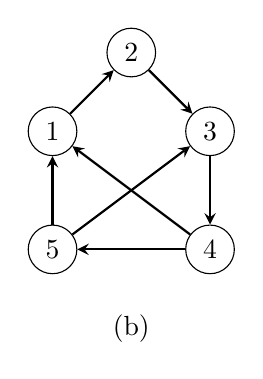
\begin{tikzpicture}
\node (lb) at (1, -1) { (b) };
    \begin{scope}[every node/.style={circle,draw}]
    \node (v4) at (2,0) { 4 };
	\node (v3) at (2,1.5) { 3};
    \node (v1) at (0,1.5) { 1 };
    \node (v5) at (0,0) { 5};
    \node (v2) at (1,2.5) { 2 };
\end{scope}
\begin{scope}[>=stealth,->,thick]
   \draw[->] (v1) edge (v2);
   \draw[->] (v2) edge (v3);
   \draw[->] (v3) edge (v4);
   \draw[->] (v4) edge (v5);
   \draw[->] (v5) edge (v1);
    \draw[->] (v5) edge (v3);
    \draw[->] (v4) edge (v1);
\end{scope}
\end{tikzpicture}
\end{center}

Just for today's recitation, we will assume that \begin{inparaenum}[(i)] \item the web graph has no self loops (we could just remove them, anyway), and \item it is strongly connected\end{inparaenum}. This is very far from being true. The real PageRank algorithm does not need this, but it will simplify things a bit for us.

\subsection*{Problem 1: A first try}

How can we use the web graph to determine the importance of a page? A natural idea is to look at the number of links to that page; the more incoming links, the higher the rank! 

\begin{enumerate}[(a)]
    \item What ranking does this give us in the two graphs above?
        \solution{The ranking is just given by the indegree of the webpage. So it works fairly well in these examples, though there are some ties.}
    \item Give some reasons why this ranking will not work well, in general. (How could you game the system?)
        \solution{If you wanted to improve the ranking of your website, you could create a whole bunch of other dummy websites which just link to your main website. This will improve its indegree, and hence its ranking. This approach would never survive the advertisers...}
\end{enumerate}

\subsection*{Problem 2: PageRank}

Let's try something more sophisticated. We would like links from ``important'' webpages to count more than links from unimportant ones. But this sounds self-referential, since ``importance'' is what we're trying to determine!

Let's try an iterative process.
Let's give each webpage a million dollars (!). On the hour, each webpage does the following: it takes all its money, divides it equally amongst the webpages it links to, and sends it along to those pages. The process continues, and we hope that things settle down eventually, so that after a while the amount of money a given webpage has stays essentially constant. We then say that the importance (or PageRank) of the webpage is how much money it ends up with.
\begin{center}
\end{center}

\begin{enumerate}[(a)]
\item Consider graph (a) shown earlier. Suppose we have $x_i$ millions of dollars at vertex $i$. Find a formula for the amount of money (in millions) $x'_i$ at each node $i$ after 1 hour.
\solution{
    \begin{align*}
        x_1' &= x_3/2\\
        x_2' &= x_1/2 + x_3 / 2\\
        x_3' &= x_1/2 + x_2.
    \end{align*}
}
\item Figure out a formula for the amount of money $x^{(n)}_i$ (in millions) that node $i$ has after $n$ hours. Prove that your formula is correct using induction. \emph{Hint: the formula for $x_3^{(n)}$ is $\tfrac13\left(4 - (-\tfrac12)^n\right)$; this should help you get started.}
    %Hence, prove that after $n$ hours, the amount of money $x^{(n)}_i$ (in millions) at node $i$ is:
\solution{
    The formula is:

    \begin{align*} x^{(n)}_1 &= \tfrac13\left(2+(-\tfrac12)^n\right)\\
                     x^{(n)}_2 &= 1\\
                     x^{(n)}_3 &= \tfrac13\left(4 - (-\tfrac12)^n\right).
\end{align*}
    Use induction on $n$. 
    
    Base case: it is true for $n=0$, since the formulae yield $x_i^{(0)} = 1$ for $i=1,2,3$.

    \newcommand{\xn}[1]{x^{(#1)}}
    Suppose the formula holds for $n$. Applying the previous part, we see that
    \begin{align*}
        \xn{n+1}_1 &= x^{(n)}_3 / 2 =  \tfrac13\left(2+(-\tfrac12)^{n+1}\right)\\
        x^{(n+1}_2 &= \xn{n}_1/2 + \xn{n}_3/2 = 1\\
        \xn{n+1}_3 &= \xn{n}_1/2 + \xn{n}_2 =  \tfrac{1}{2}\tfrac13\left(2+(-\tfrac12)^n\right) + 1\\
                   &=  \tfrac13\left(4 - (-\tfrac12)^{n+1}\right).
    \end{align*}
    Thus the formula holds for all $n \geq 0$ by induction.
}
\item What happens as $n$ goes to infinity?  Hence determine the PageRank of the webpages.
\solution{Since $(-1/2)^n \to 0$ as $n \to \infty$, we obtain the limiting amounts $p_1 = 2/3$, $p_2 = 1$ and $p_3 = 4/3$.}

\item The formula for $\vec{x}'$ in terms of $\vec{x}$ can be written as a matrix product: $\vec{x}' = W\vec{x}$, for some matrix $W$ (we'll call this the \emph{update matrix}). Determine $W$.
    \solution{
    \[ W = \begin{pmatrix} 0 & 0 & 1/2\\ 1/2 & 0 & 1/2\\ 1/2 & 1 & 0 \end{pmatrix}. \] }
\item Check that it satisfies the equation $\vec{p} = W\vec{p}$, where $\vec{p}$ is the vector of PageRanks\footnote{We snuck in some linear algebra; some of you may recognize that $p$ is an eigenvector of $W$, with associated eigenvalue $1$.}. (In other words, $p_i$ is the PageRank of page $i$.)
\end{enumerate}
This last fact is true in general: for any strongly connected web graph $G$, with $W$ being its update matrix, the equation
\begin{equation}\label{eq:eig} \vec{p} = W\vec{p} \end{equation}
is satisfied by the vector $\vec{p}$ of PageRanks. We won't prove this, but assume this for the next question.

\begin{center}
\end{center}
\begin{enumerate}[(a)]
        \setcounter{enumi}{5}

    \item Determine the update matrix $W$ for the web graph (b) shown earlier. Hence determine the PageRank vector $\vec{p}$ by finding a non-zero solution to \eqref{eq:eig}. \emph{(The solution is not unique; but if you add the requirement that, e.g., $p_1 = 1$, then it will be unique).}
    \solution{
        \[ W = \begin{pmatrix} 0 & 0 & 0 & 1/2 & 1/2\\ 1 & 0 & 0 & 0 & 0\\ 0 & 1 & 0 & 0 & 1/2\\ 0 & 0 & 1 & 0 & 0\\ 0 & 0 & 0 & 1/2 & 0\end{pmatrix}. \]
        The equation $\vec{p} = W\vec{p}$ yields the following system of equations:
        \begin{align*}
            p_1 &= p_4/2 + p_5/2\\
            p_2 &= p_1\\
            p_3 &= p_2 + p_5/2\\
            p_4 &= p_3\\
            p_5 &= p_3/2.
        \end{align*}
        Putting in the normalizing constraint that $p_1 = 1$, we can solve this system to obtain
        \[ p_1 = p_2 = 1 \qquad p_3 = p_4  = 4/3 \qquad p_4 = 2/3. \]
    }
%\item Show that the PageRank of any webpage in a webgraph $G$ that is strongly connected is strictly positive. What if $G$ is not strongly connected?
\end{enumerate}

\end{document}
